\documentclass[a4paper,11pt,oneside]{article}

\usepackage{amsmath,amssymb,epsfig}
\usepackage[T1]{fontenc}
\usepackage{ae,aecompl}
\usepackage{url}
\usepackage{subfigure}
\addtolength{\voffset}{-1cm}
\addtolength{\hoffset}{-1cm}
\setlength{\parindent}{0in}
\addtolength{\textwidth}{1.8cm}
\addtolength{\textheight}{1cm}
\addtolength{\parskip}{.5cm}

% Example definitions.
% --------------------
\def\x{{\mathbf x}}
\def\X{{\mathbf X}}
\def\u{{\mathbf u}}
\def\U{{\mathbf U}}
\def\x{{\mathbf x}}
\def\s{{\mathbf s}}
\def\A{{\mathbf A}}
\def\y{{\mathbf y}}
\def\W{{\mathbf W}}
\def\w{{\mathbf w}}
\def\B{{\mathbf B}}
\def\D{{\mathbf D}}
\def\a{{\mathbf a}}
\def\D{{\mathbf D}}
\def\P{{\mathbf P}}
\def\n{{\mathbf n}}
\def\V{{\mathbf V}}
\def\R{{\mathbf R}}
\def\I{{\mathbf I}}
\def\M{{\mathbf M}}
\def\sech{{\mathrm{sech}}}
\def\L{{\cal L}}
\def\Cum{{\rm{Cum}}}
\def\var{{\rm{var}}}
\def\T{{\mathbf T}}
\def\C{{\mathbf C}}
\def\tf{{\emph{t-f}}}


% Title.
% ------
\title{Discrete-Time Signals and Systems in the z-Domain}
%
% Author and date.
% ---------------
\date{\today}
\author{Germ\'an G\'omez-Herrero, \url{http://germangh.com}}



\begin{document}
\maketitle


\textbf{NOTE:} This document is a brief summary (a cheatsheet, actually) of Chapter 6 from the textbook \emph{Digital Signal Processing}, by S. K. Mitra. 



\begin{itemize}

\item The z-transform of a given sequence $g[n]$ is defined as:

\[
G(z) = \sum_{n=-\infty}^{\infty}g[n]z^{-n}
\]

where $z=\textrm{Re}(z)+j\textrm{Im}(z)$ is a complex variable. In general, converges only for an anular region of the z-plane, i.e. the Region of Convergence (ROC) of a z-transform is $R_{1}<|z|<R_{2}$ where $0\leq R_{1}<R_{2}\leq\infty$. In some occassions the ROC includes also the points $z=0$ and $z=\infty$. Of course, you should remember that the modulus of a complex number is given by $|z|=\sqrt{\textrm{Re}(z)^2+\textrm{Im}(z)^2}$. 

\item Notice that when we say that a z-transform, e.g. $G(z)$, diverges for $z=\lambda$ this means that $G(\lambda)=\infty$. Those values $\lambda_1,\lambda_2,...,\lambda_{N}$ for which a Z-transform diverges (i.e. $G(\lambda_i)=\infty \;\forall i=1,2,...,N$) are called \emph{poles} of $G(z)$. Indeed, the definition of ROC forces all the poles to be outside the ROC.

\item By contrary, those values $\epsilon_1,\epsilon_2,...,\epsilon_M$ for which $G(z)$ becomes zero (i.e. $G(\epsilon_i)=0 \;\forall i=1,2,...,N$) are called \emph{zeros} of $G(z)$. Indeed, all the zeros of a Z-transform have to be inside its ROC since $G(\epsilon_i)\neq \infty$.


\item Let us compute the z-transform $X(z)$ of the causal sequence $x[n]=\alpha^{n}\mu[n]$ where $\mu[n]$ is the unit step sequence:

\begin{equation}\label{eq1}
X(z)=\sum_{n=-\infty}^{\infty}\alpha^n\mu[n]z^{-n}=\sum_{n=0}^{\infty}(\alpha z^{-1})^n
\end{equation}

Remember that the sum $\sum_{n=0}^{\infty}r^n$ converges to $\frac{1}{1-r}$ only if $|r|<1$. Otherwise the sum diverges (becomes $\infty$). So this means that Eq.~\ref{eq1} becomes:

\begin{equation}
X(z)=\left\{
\begin{array}{lll}
\frac{1}{1-\alpha z^{-1}} &\quad & \textrm{if} \quad |\alpha z^{-1}|<1 \Leftrightarrow |z|> |\alpha|\\
\infty &\quad& \textrm{if} \quad |\alpha z^{-1}|\geq 1  \Leftrightarrow |z|\leq |\alpha|
\end{array}
\right.
\end{equation}

Instead of expressing the $X(z)$ like above we usually express it by saying that the z-transform of $x[n]$ is $\frac{1}{1-\alpha z^{-1}}$ and its \emph{region of convergence (ROC)} is $|z|>\alpha$. Moreover, you can plot the region of convergence in an \emph{Argand diagram}\footnote{An \emph{Argand diagram} is just a type of cartesian representation of a complex number in which the vertical axis is the imaginary axis and the horizontal axis is the real axis. See Fig.~\ref{arganddiagram} for an example of an Argand diagram.}.


\item It is very important to realize that a the expression of a z-transform is meaningless without its ROC. This is because different sequences in the time domain might have exactly the same expression in the z-domain but with different ROCs. Therefore knowledge of the ROC is necessary in order to have a 1-to-1 relation between the time-domain and the z-domain, which is what makes inversion of the z-transform possible. For instance the z-transform of the sequence $y[n]=-\alpha^n\mu[-n-1]$ is:

\begin{equation}
Y(z)=\left\{
\begin{array}{lll}
\frac{1}{1-\alpha z^{-1}} &\quad & \textrm{if} \quad |\alpha^{-1} z|<1 \Leftrightarrow |z|<|\alpha|\\
\infty &\quad& \textrm{if} \quad |\alpha^{-1} z|\geq 1 \Leftrightarrow |z|\geq |\alpha|
\end{array}
\right.
\end{equation}

notice that despite the appearances, $Y(z)$ and $X(z)$ are different because their ROCs are different. The ROC of $X(z)$ are all the points in the z-plane exterior to a circunference of radius $|\alpha|$ (including the point $z=\infty$) whereas the ROC of $Y(z)$ are all the points interior to that circunference (including $z=0$).

\item To make things easier for you in the exam you should memorize the z-transforms of the sequences in Table~\ref{basicztransforms}, which you will need all the time when computing inverse Z-transforms.

\begin{table}
\centering
\begin{tabular}{ccc}
\hline
Sequence & Z-transform & ROC\\
\hline
$\delta[n]$ & 1 & $\forall z$\vspace{.2cm}\\
$\alpha^n\mu[n]$ &  $\frac{1}{1-\alpha z^{-1}}$ & $|z|>|\alpha|$\vspace{.2cm}\\
$-(\alpha)^{n}\mu[-n-1]$ & $\frac{1}{1-\alpha z^{-1}}$ & $|z|<|\alpha|$\vspace{.2cm}\\
$n \alpha^n \mu[n]=n\alpha^n\mu[n-1]$ & $\frac{\alpha z^{-1}}{(1-\alpha z^{-1})^2}$ & $|z|>|\alpha|$\vspace{.2cm}\\
$-n\alpha^n \mu[-n-1]=-n\alpha^n\mu[-n]$ & $\frac{\alpha z^{-1}}{(1-\alpha z^{-1})^2}$ & $|z|<|\alpha|$\vspace{.2cm}\\
\hline
\end{tabular}
\caption{Z-transforms and ROCs associated with several elementary sequences. Notice that the $n$ factor in $n\alpha^n\mu[n]$ cancels the expression for $n=0$ which makes such expression equivalent to $n\alpha^n\mu[n-1]$. For the same reason $-n\alpha^n \mu[-n-1]=-n\alpha^n\mu[-n]$.}
\label{basicztransforms}
\end{table}

\item You should also memorize the properties of the Z-transform in Table~\ref{propertiesz}, among which the shifting and time-reversal properties are probably the most important ones. Do not forget to memorize (or understand) the last column of the table where it says what happens to the ROC under any of these transformations.


\begin{table}
\centering
\begin{tabular}{cccc} 
\hline
Sequence & Z-transform && ROC\\
\hline
$g[n]$ & $G(z)$ && $R_g$\vspace{.2cm}\\
$h[n]$ & $H(z)$ && $R_h$\vspace{.2cm}\\
\hline
$g^*[n]$ & $G^*(z^*)$ && $R_g$\vspace{.2cm}\\
$g[-n]$ & $G(\frac{1}{z})$ && $\frac{1}{R_g}$\vspace{.2cm}\\
$\alpha g[n]+\beta h[n]$ & $\alpha G(z) + \beta H(z)$ && $\textrm{includes } R_g\cap R_h$\vspace{.2cm}\\
$g[n-n_0]$ & $z^{-n_0}G(z)$ && $R_g\;\textrm{except maybe } z=0\;\textrm{or } z=\infty$\vspace{.2cm}\\
$\alpha^n g[n]$ & $G(\frac{z}{\alpha})$ && $|\alpha|R_g$\vspace{.2cm}\\
$ng[n]$ & $-z\frac{dG(z)}{dz}$ && $R_g\;\textrm{except maybe } z=0\;\textrm{or } z=\infty$\vspace{.2cm}\\
$g[n]\otimes h[n]$ & $G(z)H(z)$ && $\textrm{includes } R_g\cap R_h$\vspace{.2cm}\\
\hline
\end{tabular}
\caption{Most important properties of the Z-transform. $R_g$ denotes the region of the z-plane $R_{g-}<|z|<R_{g+}$ and $R_h$ denotes the region $R_{h-}<|z|<R_{h+}$. Then $1/R_g$ denotes the region $1/R_{g+}<|z|<1/R_{g-}$.}
\label{propertiesz}
\end{table}

\item From Table~\ref{basicztransforms} and Table~\ref{propertiesz} follows the additional properties in Table~\ref{propertiesz2}. Using these three tables one can compute the ROC of the Z-transform of many sequences without actually computing the Z-transform of the sequence. This is very often an exam problem. For instance if they ask you to find the ROC of the Z-transform of the sequence:

\[
x[n] = \left\{
\begin{array}{lll}
\left(\frac{1}{2}\right)^n &&\textrm{if}\quad 2\leq n \leq 7\\
0&&\textrm{otherwise}\\
\end{array}
\right.
\]

one can see that the sequence $x[n]$ is of finite duration and therefore its ROC must be the whole z-plane except maybe $z=0$ and/or $z=\infty$ (Table~\ref{propertiesz2}). Moreover, the sequence is different of zero for some positive values of $n$ (that is, $M>0$ in Table~\ref{propertiesz2}) which means that the Z-transform will contain negative powers of $z$ and, therefore, will have one or several poles in $z=0$, i.e. the point $z=0$ will be outside the ROC. At the same time, our sequence is always zero for any negative values of $n$ (so $N>0$ in Table~\ref{propertiesz2}) and as a result the Z-transform will not contain positive powers of $z$ which will avoid the existence of poles at $z=\infty$. As a result of all this, the ROC of this sequence is $0<|z|$.

Consider now the ROC of the sequence $y[n]=3^n\mu[-n]$. We can rewrite this sequence as $y[n]=(3^{-1})^{-n}\mu[-n]$. Because of Table~\ref{basicztransforms} we know that the ROC of sequence $(3^{-1})^n\mu[n]$ is $|z|>3^{-1}$. Then, using the time-reversal property in Table~\ref{propertiesz} we obtain that the ROC of $y[n]=3^n\mu[-n]$ is $|z|<\frac{1}{3^{-1}}\Leftrightarrow |z|<3$. 

\begin{table}
\centering
\vspace{1cm}
\begin{tabular}{lll}
\hline
\hline
Property of $g[n]$ & & ROC of $G(z)$\\ 
\hline
\hline
&&\vspace{-0.3cm}\\
Finite length&&All z-plane except\\
$g[n]=0\;\forall n>M\;\forall n<N$&&except $z=0$ if $M>0$\\
&&except $z=\infty$ if $N<0$\vspace{.2cm}\\
\hline
Causal & \quad & $R_{g-}<|z|$\\
$g[n]=0\;\forall n<0$&&\vspace{.2cm}\\
\hline
Anticausal& \quad & $|z|<R_{g+}$\\
$g[n]=0\;\forall n>0$ &&\vspace{.2cm}\\
\hline
Left-sided &\quad & $0<|z|<R_{g+}$\\
$g[n]=0\;\forall n>N\;\textrm{with } N>0$&&\vspace{.2cm}\\
\hline
Right-sided &\quad & $R_{g-}<|z|<\infty$\\
$g[n]=0\;\forall n<M\;\textrm{with } M<0$&&\vspace{.2cm}\\
\hline
\end{tabular}
\caption{Properties of the ROC of the Z-transform of a sequence depending on the span of the sequence in time-domain.}
\label{propertiesz2}
\end{table}
\vspace{1cm}


\item A discrete-time LTI system is often characterized by a linear constant coefficient difference equation of the form:

\begin{equation} \label{diffeq}
\sum_{k=0}^{N}d_{k}y[n-k]=\sum_{k=0}^{M}p_kx[n-k]
\end{equation}


Using the shifting property of the Z-transform (see Table~\ref{propertiesz}) it is obvious that Eq.~\ref{diffeq} is represented in the Z-domain by:

\[
\left(\sum_{k=0}^{N}d_k z^{-k}\right)Y(z)=\left(\sum_{k=0}^{M}p_k z^{-k}\right)X(z)
\]

and then the \emph{transfer function} of the given LTI system is defined as:

\begin{equation}\label{rationalz}
H(z)=\frac{Y(z)}{X(z)}=\frac{\sum_{k=0}^{M}p_k z^{-k}}{\sum_{k=0}^{N}d_k z^{-k}}
\end{equation}

The transfer function of the system can also be written in terms of zeros and poles as:

\[
H(z)=\frac{p_0}{d_{0}}z^{N-M}\frac{\prod_{k=1}^{M}(z-\epsilon_k)}{\prod_{k=1}^{N}(z-\lambda_k)}
\]

where $\epsilon_1,\epsilon_2,...,\epsilon_k$ are the zeros and $\lambda_1,...,\lambda_k$ are the poles of $H(z)$. Using $H(z)$ one can characterize an LTI system in many ways. For instance:
\begin{itemize}
\item If the ROC of $H(z)$ includes the unit circle then the system is \emph{stable}.
\item If the ROC of $H(z)$ includes the point $z=\infty$ then the system is \emph{causal}.
\item If the ROC of $H(z)$ includes the unit circle and the point $z=\infty$ then the system is both causal and stable. This is the same as saying that the system is \emph{realizable}.
\item A \emph{realizable} system $H(z)$ is said to be \emph{minimum phase} if its inverse is also realizable, i.e. if all the zeros of $H(z)$ are inside the unit circle.
\end{itemize}

\item In a system $H(z)$ is \emph{causal} (the most common case) then the ROC of $H(z)$ is  $|z|>\max_k{|\lambda_k|}$. If a system is causal we can determine if it is stable, realizable and minimum phase by simply examining the positions of the zeros and poles of $H(z)$:

\begin{itemize}
\item If all the poles are within the unit circle, i.e. if $|\lambda_k|<1 \; \forall k$, then the system will be \emph{stable} and therefore it will also be \emph{realizable}. 
\item If all the poles and all the zeros are within the unit circle, i.e. if $|\lambda_k|<1 \; \forall k$ and $|\epsilon_k|<1 \; \forall k$ then the system will be \emph{minimum phase} and therefore the inverse system $\frac{1}{H(z)}$ will be realizable (i.e. causal and stable).
\end{itemize}

\item The inverse of the transfer function is the impulse response of the system: $h[n]=Z^{-1}\left\{H(z)\right\}$. So it is important to be able to invert rational Z-transforms as the one in Eq.~\ref{rationalz}. This is one of the most important parts of this chapter. Basically the idea is to manipulate the rational expression $H(z)$ so that it will become just a summation of elementary terms having expressions as the ones given in Table~\ref{basicztransforms}. Then, using the linearity property, $H(z)$ can be inverted by inverting each of these elementary terms. An additional document is available in the course web-page where this is explained step-by-step using a practical example. Notice that inverting a Z-transform is almost always necessary in at least one (often more) of the problems of the exam.

\item Another problem that often appears in the exam is to compute the linear convolution of two sequences $x[n]$ and $h[n]$ using the Z-transform:

\[
y[n]=x[n]\otimes h[n]=Z^{-1}\left\{X(z)Y(z)\right\}
\]

\item An LTI system is fully defined by its system function $H(z)$ but you should be aware that $H(z)$ can be given in different ways:

\begin{enumerate}
\item Using a difference equation like in Eq.~\ref{diffeq}. In this case the system function can be directly obtained using Eq.~\ref{rationalz}.
\item Giving you the output of the system $y[n]$ for a given input sequence $x[n]$. In this case, the system function can be easily obtained as $H(z)=\frac{Y(z)}{X(z)}$.
\item Giving you directly either the impulse response $h[n]$ or the system function $H(z)$.
\end{enumerate}







\begin{figure}
\centering
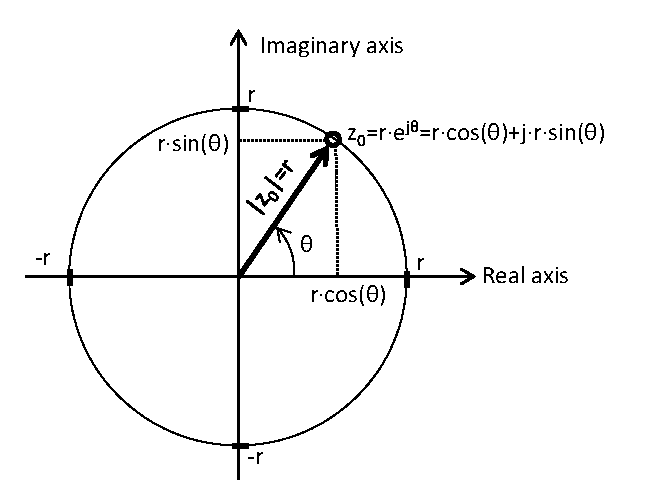
\includegraphics[width=.7\textwidth]{arganddiagram.eps}
\caption{A complex number $z_0=a+jb=r\cos \theta + jr\sin \theta=re^{j\theta}$ can be represented as a vector in an Argand diagram. The length of the depicted vector is the modulus of the complex number $|z_0|=r$. Obviously, all the complex numbers satisfying $|z|=r$ are located in a circunference of radius $r$. Then the equation $|z|>r$ describes the area strictly outside that circunference whereas the equation $|z|<r$ describes the area strictly inside that circunference. Similarly the equation $r_0<|z|<r_1$ with $r_0<r_1$ describes the anular area between a circunference of radius $r_0$ and another one of radius $r_1$.}
\label{arganddiagram}
\end{figure}


 

\end{itemize}



\end{document}